\Chapter{GENERAL DISCUSSION}\label{sec:Theme3}

Indeed, the demand for performance is increasing, even more for the software part, consequently this new technique can be used on this matter. In this context, this research aims to demonstrate a new perspective on system analysis in the identification of performance root causes and it will be especially useful as a tool for performance improvement. \\
The proposed solution is an autonomous technique, which combines tracing and clustering, to find causes of performance issues on real programs. This research can still be relevant even software updates and obsolescence since it relies on a methodology rather than a tool. Moreover, the heuristic utilization is able to fulfill this requirement since it can be applied with different classification methods and arbitrary dimensions. \\
Considering the present status quo in tracing and performance counters, this work could be applied as it is in different environments and even integrated in a testing framework such as PARCS. Although some adaptations will need to be done in the data collection part, the main part of this research can be used other domains as well.\\
The development of better PADBI tools, Performance Anomaly Detection and Bottleneck Identification, eventually is leading towards automated mechanisms and methods and the data mining methods presented in this work aim to partially fulfill this gap.
\section{Methods comparison}
Since several methods were applied to the task and it is possible to compare them in several ways, which are summarized below.
As explained in the article the SVM model delimits an hyperplane to divide the data and as consequence is able to segregate the slow executions and fast executions, in a dichotomy way. In some scenarios, especially considering the influence of outliers, the classification can be mislead, also segregated data gives strange results.\\
 \begin{figure}[h]
          \center
          \caption{Support Vector Scenarios}
            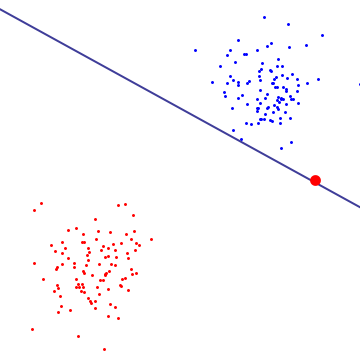
\includegraphics[width=0.50\textwidth]{figures/svm.png}
            \label{fig:svm_scenarios}
 \end{figure}
The second method, percentage classification, is an unsupervised mechanism and leads to segregation of data even if they are homogeneously distributed among the dataset. The percentage classification is interesting to be used in the scenarios similar to k-means, without the unpredictable of the original method.\\
This method is interesting when the standard deviations of the data are similar, so the result will be a reduced number of groups, even one group as result but might lead to many groups when the average distance of them is larger than a certain threshold. This method weave the solution of a specific problem to quantify the groups in a distribution, scenario 1, in the Figure 5.1. 
 
 \begin{figure}[h]
          \center
          \caption{Percentage Classification Scenarios}
            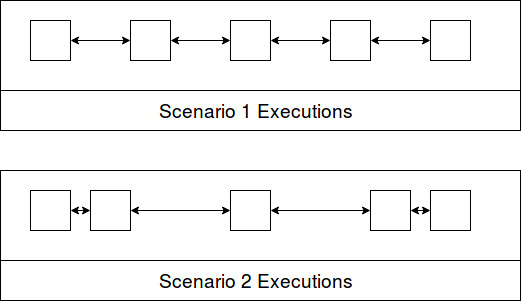
\includegraphics[width=0.90\textwidth]{figures/scenarios_percentage.jpg}
            \label{fig:scenarios_percentage}
    \end{figure}

Finally, the k-means algorithm is efficient but requires the number of groups to be used in the classification process, which cluster the data using a centroid. Still, k-means does not carry the exact same result at each run.
The k-means algorithm is specially interesting in scenarios such as: two or three main clusters. However, in scenarios where the data is homogeneously distributed and when there is just one cluster.
The scenarios described in Figure 5.2 are clear limitation of k-means algorithm. The first scenario is when the data is not suitable for this technique. In our experiments both were not found in the use cases, but could occur.\\
 
 \begin{figure}[h]
          \center
          \caption{K-means Scenarios }
            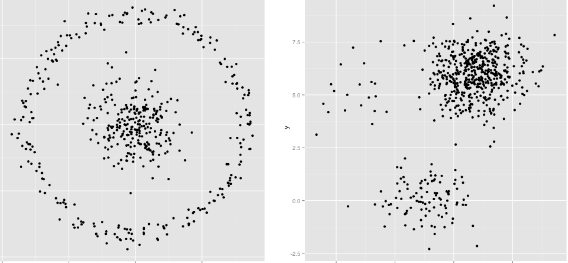
\includegraphics[width=0.90\textwidth]{figures/scenarios_k.png}
            \label{fig:scenarios_k}
    \end{figure}

The methods described on this work summarize a series of methods to measure differences among groups of execution. The data mining methods, i.e. SVM, k-means and percentage classification. On the other hand, the statistical method used in the solution can provide a relative comparison of the performance among the groups to specific indicate the metrics as a cause for issues.\\
The statistical tools can also be used to detect regressions, as the collaboration \cite{google_releases} showed, using confidence Interval to find regressions among Chromium releases. 
As final remarks in the comparison is whether the groups are well defined and where the anomalies are just not a new pattern in the data as listed in \cite{Chandola2009ADS15418801541882}. In this matter, each grouping technique, such as the percentage grouping, have its own borders definition.
\section{Results discussion}
The results were able to indicate specific metrics that might be used to improve a software performance. The solution can be used in two ways: as a detection tool or as analysis tool. In other words, in some cases the solution is able specifically to demonstrate where should be done the corrections in other cases the solution will give a guideline to a specific metric of the issue, i.e. a metric guidance that can be used by the developer to find the source code.\\
The example of OpenCV, it was possible to reduce the number of commits using the result in a specific function. However, it was necessary to consider the code of the application to do a complete analysis.\\
In other cases, the longer runs were related to specific metrics, e.g. cache misses, and the groups comparison was able to identify this information. The versions could then be compared considering this information, so the regressions test can be properly done.
\section{Metrics collision}
During the experiments we found that an overhead was added in due to the use of several performance metrics in the tracing method. Therefore, instead of recording all the metrics at the same time, it is possible to used an experiment setup that can be used to infer the influence of different metrics in a application. This setup is similar to psychology tests. \\
This method is not presented in the paper, since we were able to trace the applications with all the metrics enabled. Using the cross validation setup, the results can be summarized in the tables below:
\begin{table}[h]
\centering
\caption{Table Metric Association}
\label{tab:table1}
\begin{tabular}{lll}
\hline
Metric A              & Metric B   &     Metric C        \\ \hline
enabled & - & enabled \\ \hline
- & enabled & enabled \\ \hline
enabled & enabled & - 
\end{tabular}
\end{table}
 
Considering that the results are the following Table \ref{tab:table2}, the cross where the impact of BC is 40 percent and the impact of AB is 10 percent, the deduced impact of C must be no less than 20 percent.
    
\begin{table}[h]
\centering
\caption{Table Group Impact}
\label{tab:table2}
\begin{tabular}{ll}
\hline
Groups             &    Impact   \\ \hline
AB & 10 percent impact \\ \hline
AC & 40 percent impact \\ \hline
BC & 30 percent impact
\end{tabular}
\end{table}

It is possible therefore to construct an association rule to simplify this process and avoid tracing overhead unnecessarily.
\section{Auto clustering discussion}
Considering the models shown above, we chose to develop a non-supervised method, a.k.a auto clustering. The possibility to use an automated approach is more interesting for us in comparison with a non-automated methods, mainly because we aim not to use the data to train the model. \\
Therefore, we implemented a version of comparative k-means using the SSE (sum of square errors) variability information, plus a heuristic evaluation. This technique can be used for an arbitrary dimension of since the amount of difference, SSE (sum of squared error), can be calculated on those cases.  Some limitations apply on this approach and it is possible to use Gaussian Mixture Model to overcome them, as elaborated in \cite{gaussian}.\\
Since the SSE drops considerably between one group and two groups, we need always to consider more than two groups, otherwise the chosen gap will be two groups.
From the perspective of the Elbow method, also called silhouette method, which in fact is just of of the criteria that can be used to find the best k, as the calinski criterion as described in \cite{calinski}. This approach, Calinski-Harabasz,  is used in \cite{cluster} to specifically determine the number of clusters.\\
The used approach can also be compared with the x-means clustering technique, where the best results are kept to be compared.A more complete approach could be done using the gap statistical calculation, which uses calculation of within cluster dispersion, as described in \cite{gap_statistical}.
The next step would be to use an agglomerative clustering technique, which is an bottom up technique where each observation.

\section{Performance Counters}
The first highlight in the research are the performance counters used are limited to the counters in Perf. The more addition, the more overhead is added, so the use cross-validation scheme. 
Depending on the quantity of different metric counters, the process of grouping will increase its complexity, even hundreds of metrics as expressed in \cite{cluster}. \\
Besides, considering hundreds of metrics, a pair-wise analysis done in the groups comparison could be a restriction, consequently another a control chart could be used.
    
\section{Data structure evaluation}
We used two dynamic structures in the solution, a calling context tree with metrics, i.e. ECCT but also a dynamic call tree with metrics, i.e. EDT instead of a ECCT. 
The main difference resides in the summarized purpose of the ECCT, which is used in previous literature. Although the EDT has much longer size comparatively, the use of EDT is to avoid the addition of a pre-processing phase in the comparison of the internal nodes, that is, when comparing small portions of a software application, where an entire tree is unnecessary, the use of a EDT can be more suitable.\\
Those two dynamic structures, as any other tree, can be analyzed comparatively in two specific ways: the topological organization of the structure and the weights of the nodes. \\
The first approach can be used to compare differences among software, specifically targeting the profiling approaches. This strategy can be used in terms of tracing mining in kernel space if a pattern approach is used to automatically delimit the entries and exits of the nodes.\\
The second approach is the used in this research and consists of comparison of weights of nodes of similar trees. In this approach, the weights are the hardware and software performance metrics, e.g. page-faults and cache-misses.
\section{Usage}
This tool has various situations where the standard profiling is not suitable and the tracing requires analysis, for example with large data traces.
An unequivocal example of real utilization of this tool are regressions tests, as shown in the use cases of OpenCV and cache-misses. Though the proposed solution can be used to detect regressions, it is suitable as a diagnosis tool, since it can indicate root cause.\\
The solution presented in this research could be integrated to PARCS or even in a similar framework, while the performance metrics are compared in each version and see the patterns, since the mining technique have a complementary approach that compares the weights of the nodes, instead of the topological structure. \\
Although not explored, it is possible to use this work for developing enhanced trees, ECCTs or EDTs, in the kernel side of the system and applying the same comparison techniques explored here, it is possible to mine data from it.
\section{Visualization Tools}
The Red Grey Green Differential, RGG, suggested in the work can reduce the ambiguity of the similar executions, which would have the same color although they had different performances comparatively. \\
This different implementation, in comparison to the standard Differential Flame Graph, will reduce the analysis time by avoiding the verification of the equal time use cases. In terms of groups of event or profiling data in general.\\
We conclude this research through an evaluative summary of the contribution by considering several aspects of the proposed solution. First, we present a summary of the work, then, the objectives attainment, this is followed by the limitations of our solution and recommend future improvements.

